\begin{frame}{circle constructions}
\begin{enumerate}
\conti 
\item Draw a circle with centre B and radius 6. If C be a point 10 units away from its centre,construct the pair of tangents AC and CD to
the circle.
\seti
\end{enumerate}
\textbf{Solution:}  
\begin{itemize}
\item Draw a circle with radius r=6cm centre B.
\item Apply Baudhayana theorem ABC and BCD to get AC,DC distance and find A and D coordinates.$$B=\begin{pmatrix}
0 \\ 0
\end{pmatrix}
C=\begin{pmatrix}
10 \\ 0
\end{pmatrix} 
A=\begin{pmatrix}4.5\\3.96\end{pmatrix} D=\begin{pmatrix}4.5\\-3.96\end{pmatrix}$$

\end{itemize}
\end{frame}
\begin{frame}
\begin{figure}[!ht]
\resizebox{0.8\linewidth}{!}
{
\begin{tikzpicture}[scale =1.5,>=stealth,point/.style = {draw, circle, fill = black, inner sep = 1pt},]
\draw (0,0)circle (6cm);
\node (C) at (10,0)[point,label=above :$\textbf{C(10,0)}$] {};
\node (A) at (4.5,3.96862697)[point,label=below :$\textbf{A(4.5,3.96)}$] {};
\node (B) at (0,0)[point,label=below :$\textbf{B(0,0)}$] {};
\node (D) at (4.5,-3.96862697)[point,label=below :$\textbf{D(4.5,-3.96)}$] {};
\draw (B)--node[below] {$\textbf{10cm}$}(C)--(D)--(B);
\draw (B)--(A)--(C);
\end{tikzpicture}



}
\caption{Circle with tikz}
\label{fig:foo}
\end{figure}
\end{frame}
\begin{frame}
\begin{figure}[!ht]
\resizebox{0.5\linewidth}{!}
{
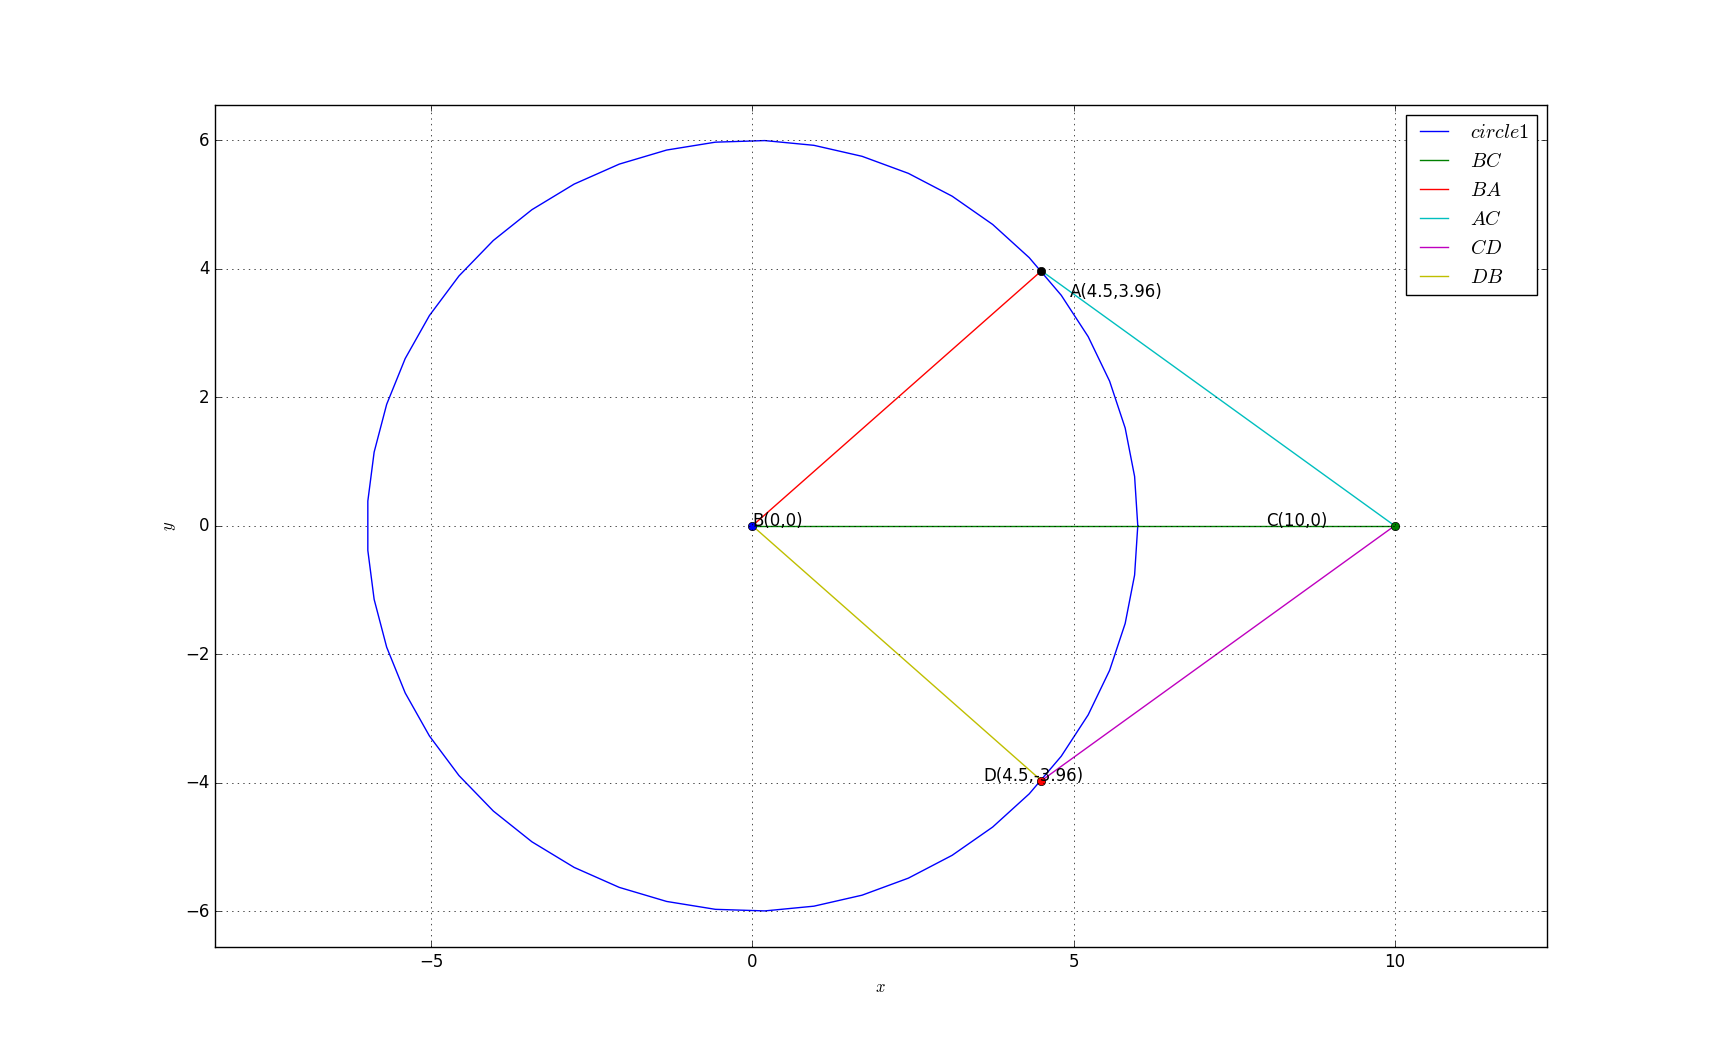
\includegraphics[scale=1.5]{./figs/circles/circle_constr.png}
}
\caption{Circle with python}
\label{fig:foo}
\end{figure}
\begin{itemize}
\item \textbf{python code :}\url{https://github.com/d-DP/geometryy/blob/master/codes/circles/circle_constr.py}\\
\item \textbf{tikz :}\url{https://github.com/d-DP/geometryy/blob/master/figs/circles/circle_constr.tex}
\end{itemize}
\end{frame}